\section{Verzerrungsmodell}

\subsection{Modelle in der Lensfun-Datenbank}

\subsection{Implementierung}

Die Klasse \texttt{DistortionCamera} implementiert die Linsenverzeichnung. Dabei werden die Richtungen der ausgesandten Strahlen relativ zum "Referenzmodell Lochkamera" modifiziert, sodass die Verzeichnung durch die unperfekte Linse im gerenderten Bild sichtbar wird. Der Raytracer ruft zum Erzeugen der Strahlen für das Rendern eines Bildes die Klassenmethode \texttt{GenerateRay} auf. Dies passiert für jeden Pixel des zu erzeugenden Bildes mindestens einmal\footnote{Der verwendete Sampler gibt vor, wie häufig und auf welche Art und Weise für ein Pixel Strahlen generiert werden.}. Die Berechnung der Strahlrichtung in Abhängigkeit der betrachteten Pixelkoordinaten erfolgt also in \texttt{GenerateRay}.

\subsubsection{Konzept ( Warum muss man invertieren? )}

Das Lochkamera-Modell geht von einer infinitesimal kleinen Blendenöffnung aus. Einfallende Lichtstrahlen, die auf die Öffnung treffen, bewegen sich ungehindert in ihre Ausbreitungsrichtung weiter und treffen an einem Punkt $p_1$ auf den Kamerasensor (siehe blauer Strahl in Abbildung \ref{fig:model}). Eine Linsenverzerrung kann nun qualitativ so modelliert werden, dass der einfallende Lichtstrahl an der Öffnung der Lochblende in einem bestimmten Maße abgeknickt wird und stattdessen an einem anderen Punkt $p_2$ auf den Sensor auftrifft (roter Strahl). Die Funktion, die die normalisierten Pixelkoordinaten des unverzerrten Punktes $p_1$ auf die des verzerrten Punktes $p_2$ abbildet, bezeichnen wir mit $f: [0,1] \rightarrow [0,1]$.
\begin{figure}[h]
	\centering
	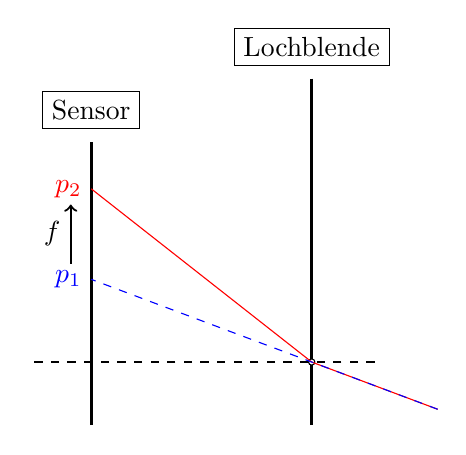
\begin{tikzpicture}[scale=0.4]
	% sensor
	\draw[very thick] (-7,-2) -- (-7, 7);
	% lochblende
	\draw (0,0) circle [radius=0.1];
	\draw[very thick] (0, -2) -- (0, -0.1);
	\draw[very thick] (0, 9) -- (0, 0.1);
	%optische Achse
	\draw[thin, dashed] (2, 0) -- (-9, 0);
	%abgelenkter Lichtstrahl
	\draw[red] (4, -1.5) -- (0, 0) -- (-7, 5.5) node[left] {$p_2$};
	%durchgehender Lichtstrahl
	\draw[blue, dashed] (4, -1.5) -- (-7, 21/8) node[left] {$p_1$};
	%Verzeichnungspfeil
	\draw[->, thick] (-7.65, 21/8 + 0.5) -- (-7.65, 65/16) node[left] {$f$} -- (-7.65, 5) ;
	%Beschriftung
	\node[draw] at (-7, 8) {Sensor};
	\node[draw] at (0, 10) {Lochblende};
	\end{tikzpicture}
	\caption{Vereinfachtes Verzerrungsmodell in 2D. Der rote von rechts einfallende Lichtstrahl wird durch die Linse abgelenkt. In blau ist der Weg dargestellt, den der Strahl nach dem Lochkamera-Modell nehmen würde. Die gestrichelte Linie zeigt die optische Achse. Die Abbildung zwischen Lochkamera-Modell und Modell mit Verzerrung ist mit $f$ bezeichnet.}
	\label{fig:model}
\end{figure}
Ein Raytracer, der eine solche Linsenverzerrung berücksichtigen soll, muss also bei der Erzeugung der Strahlen für einen gegebenen Punkt von dem Lochkamera-Modell aus Abschnitt \ref{sec:pinhole} abweichen. Allerdings gibt es für jeden Punkt $p$ auf dem Sensor einen Punkt $p'$, deren zugeordneter Strahl \emph{nach dem Lochkamera-Modell} dem Strahl entspricht, der \emph{nach dem Verzerrungsmodell} $p$ zuzuordnen ist.
In Abbildung \ref{fig:model} ist $p = p_2$ und $p' = p_1$. Da $f(p_1) = p_2$ ist, kann damit $p'$ durch Anwenden der inversen Verzerrungsfunktion $g = f^{-1}$ mit $p' = g(p)$ gefunden werden. Der Strahl für $p$ kann dann einfach nach dem Lochkamera-Modell berechnet werden, indem $p = p'$ gesetzt wird.

Damit ergibt sich für die Implementierung die Anforderung, dass bei einer vorgegebenen Verzerrungsfunktion $f$ vor Beginn des Rendering die Inverse Funktion bestimmt werden muss. Da für die in der Lensfun-Datenbank verwendeten Modelle keine einfache analytische Inverse gefunden werden kann, wird ein numerischer Ansatz verfolgt. Dazu werden zunächst Werte von $f$ für eine Reihe von $r_i$ im erlaubten Bereich bestimmt. Die Inverse wird dann als Polynom mittels des Least Squares Verfahrens angenähert.


\subsubsection{Least Squares}

Die Methode der kleinsten Quadrate (engl.: \emph{Least Squares}, kurz LS) stellt ein Verfahren, zu einer gegebenen Menge an Punkten eine Funktion zu finden, die eine mögliche unbekannte Gesetzmäßigkeit hinter der Lage der Punkte annähert \cite{lsq_wolfram}.

Sei $P = \{(x_1, y_1), (x_2, y_2), ..., (x_N, y_N)\}$ die Menge der bekannten Punkte mit $x_i, y_i \in R$. Man nimmt nun an, dass zwischen x und y ein funktionaler Zusammenhang bestehe, der durch $M$ reelle Parameter $a_j$ bestimmt wird. Damit lässt sich $y_i = f(x_i; \overrightarrow{a})$ schreiben, wobei $\overrightarrow{a} \in R^M$ die Parameter zusammenfasst. LS versucht nun, den unbekannten Parametervektor so zu ermitteln, dass die Summe der quadratischen Abweichungen $S^2$ minimiert wird:
\begin{equation}
\begin{split}
\overrightarrow{a} = \argmin_{\overrightarrow{a} \in R^M} \{ S^2 \}, \quad
S^2 =  \sum_{i=1}^{N} (y_i - f(x_i, \overrightarrow{a})^2)
\end{split}
\label{eq:opt}
\end{equation}
Setzt man für $f$ ein Polynom vom Grad $k$ an, so ist $M = k+1$ und
%\begin{equation}
\begin{gather}
f(x_i, \overrightarrow{a}) = a_0 + a_1 x_i + \dots + a_k x_i^k = \sum_{j = 0}^{k} a_j x_i^j %\\
%S^2 =\sum_{i = 1}^{N} (y_i - \sum_{j = 0}^{k} a_j x^j)^2
\end{gather}
%\end{equation}
Für das Minimum müssen die partiellen Ableitungen nach allen Parametern null sein.
\begin{equation}
\frac{\partial S^2}{\partial a_l} = -2 \sum_{i=1}^{N}(y_i - a_0 + a_1 + \dots + a_k x^k) x^l = 0, \quad 0 \leq l \leq M
\end{equation}
	%Damit ist das folgende Gleichungssystem zu lösen:
	%\begin{gather}
	%\begin{bmatrix}
	%	M & \sum_{i=1}^{M}x_i &  \dots  & \sum_{i=1}^{M} x_i^k \\
	%	\sum_{i=1}^{M} x_i & \sum_{i=1}^{M} x_i^2 & \dots  & \sum_{i=1}^{M} x_i^{k+1} \\
	%	\vdots & \vdots & \ddots & \vdots \\
	%	\sum_{i=1}^{M} x_i^k & \sum_{i=1}^{M} x_i^{k+1} & \dots  & \sum_{i=1}^{M} x_i^2k
	%\end{bmatrix}
	%\cdot
	%\begin{bmatrix}
	%a_0 \\ a_1 \\ \vdots \\ a_k
	%\end{bmatrix} =
	%\begin{bmatrix}
	%\sum_{i=1}^{M} y_i \\ \sum_{i=1}^{M} x_i y_i \\ \vdots \\ \sum_{i=1}^{M} x_i^k y_i
	%\end{bmatrix}
	%\end{gather}
Es muss also ein Gleichungssystem gelöst werden, dass sich wie folgt darstellen lässt:
\begin{gather}
X^T \cdot X \cdot \overrightarrow{a} = X^T \cdot
\overrightarrow{y} \label{eq:solution}
\end{gather}
mit 
\begin{gather}
X =
\begin{bmatrix}
1 & x_1 & \dots & x_1^k \\
1 & x_2^k & \dots & x_2^k \\
\vdots & \vdots & \ddots & \vdots \\
1 & x_N & \dots & x_N^k
\end{bmatrix}
\text{und} \overrightarrow{y} = \begin{bmatrix}
y_1 \\ y_2 \\ \vdots \\ y_N
\end{bmatrix}
\end{gather}
Sind alle $x_i$ paarweise voneinander verschieden, so ist $X$ regulär. Daraus folgt die Regularität von $X^T \cdot X$. Damit ist das Problem unter dieser Bedingung immer eindeutig lösbar. Die Matrixgleichung \ref{eq:solution} kann somit numerisch oder direkt durch Finden von $(X^T \cdot X)^{-1}$ gelöst werden \cite{lsq_poly_wolfram}. In der Implementierung von \texttt{DistortionCamera} geschieht dies mittels LR-Zerlegung (beschrieben zum Beispiel in \cite{bronstein}).

Ist also eine Funktion $f(x)$ gegeben, so kann durch Auswahl von $N$ paarweise unterschiedlichen Werten $x_i$ im Bereich $[0,1]$ die Menge $P = \{ (x_1, y_1), (x_2, y_2), \dots, (x_N, y_N) \}, \quad y_i = f(x_i)$ erzeugt werden. Um nun die inverse Funktion per LS anzunähern, tauscht man in den Paaren in $P$ nun jeweils $x_i$ und $f(x_i)$ und führt dann das LS Verfahren wie oben beschrieben durch. Dies entspricht dem Optimierungsproblem
\begin{equation}
\begin{split}
\overrightarrow{a} = \argmin_{\overrightarrow{a} \in R^M} \{ S^2 \}, \quad
S^2 =  \sum_{i=1}^{N} (x_i - f(y_i, \overrightarrow{a})^2)\quad.
\end{split}
\end{equation}
Im Vergleich zu Gleichung \ref{eq:opt} sind also die Rollen von $x_i$ und $y_i$ getauscht.